\documentclass[12pt,oneside]{article}

%%%%%%%%%%%%%%%%%%%%%%%%%%%%
%%   Zusaetzliche Pakete  %%
%%%%%%%%%%%%%%%%%%%%%%%%%%%%
\usepackage{acronym}
\usepackage{enumerate}  
\usepackage{a4wide}
\usepackage{fancyhdr}
\usepackage{graphicx}
\usepackage{palatino}
\usepackage{blindtext}
\usepackage{multirow}
\usepackage[ruled,longend]{algorithm2e}
\usepackage{float}


%folgende Zeile auskommentieren für englische Arbeiten
\usepackage[ngerman]{babel}

\usepackage[T1]{fontenc}
\usepackage[utf8]{inputenc}
\usepackage[bookmarks]{hyperref}
\usepackage[justification=centering]{caption}
\usepackage[natbib=true,backend=bibtex,style=numeric,sorting=none]{biblatex}
\usepackage{csquotes}
\bibliography{literatur}


\renewcommand{\baselinestretch}{1.5} 
%%%%%%%%%%%%%%%%%%%%%%%%%%%%%%
%% Definition der Kopfzeile %%
%%%%%%%%%%%%%%%%%%%%%%%%%%%%%%

\pagestyle{fancy}
\fancyhf{}
\cfoot{\thepage}
\setlength{\headheight}{16pt}

%%%%%%%%%%%%%%%%%%%%%%%%%%%%%%%%%%%%%%%%%%%%%%%%%%%%%
%%  Definition des Deckblattes und der Titelseite  %%
%%%%%%%%%%%%%%%%%%%%%%%%%%%%%%%%%%%%%%%%%%%%%%%%%%%%%

\newcommand{\JMUTitle}[9]{

  \thispagestyle{empty}
  \vspace*{\stretch{1}}
  {\parindent0cm
  \rule{\linewidth}{.7ex}}
  \begin{flushright}
    \vspace*{\stretch{1}}
    \sffamily\bfseries\Huge
    #1\\
    \vspace*{\stretch{1}}
    \sffamily\bfseries\large
    #2
    \vspace*{\stretch{1}}
  \end{flushright}
  \rule{\linewidth}{.7ex}

  \vspace*{\stretch{1}}
  \begin{center}
    
\includegraphics[width=3in]{logo} \\
    \vspace*{\stretch{1}}
    \Large Hausarbeit  \\

    \vspace*{\stretch{2}}
   \large Autor: Hannes Frey \\
    \vspace*{\stretch{1}}
    \large Betreuer:  Roland Kiefer \\[1mm]
    
    \vspace*{\stretch{1}}
    \large Stuttgart, den #6
  \end{center}
}


%%%%%%%%%%%%%%%%%%%%%%%%%%%%
%%  Beginn des Dokuments  %%
%%%%%%%%%%%%%%%%%%%%%%%%%%%%

\begin{document}

  \JMUTitle
      {Kryptowährungen }        % Titel der Arbeit
      {Funktionsweise, Chancen und Risiken}                        % Vor- und Nachname des Autors
      
      {Wirtschaftswissenschaftlichen Fakultät}  % Name der Fakultaet
      {W"urzburg 2018}                          % Ort und Jahr der Erstellung
      {31.05.2021}                              % Tag der Abgabe
      {Prof. Dr. Christian Janiesch}               % Name des Erstgutachters
      {Zweitgutachter}                          % Name des Zweitgutachters
      {Pr"ufungsdatum}                          % Datum der muendlichen Pruefung

  \clearpage

\lhead{}
\pagenumbering{Roman} 
    \setcounter{page}{1}

\tableofcontents
\clearpage

\addcontentsline{toc}{section}{\listfigurename}
\listoffigures

\addcontentsline{toc}{section}{\listtablename}
\listoftables
\clearpage

%%%%%%%%%%%%%%%%%%%%%%%%%%%%
%%  Kurzzusammenfassung   %%
%%%%%%%%%%%%%%%%%%%%%%%%%%%%
\markboth{Zusammenfassung}{Zusammenfassung}
\section*{Zusammenfassung}
\blindtext
\clearpage

%%%%%%%%%%%%%%%%%%%%%%%%%%%%
%%  Abstract   %%
%%%%%%%%%%%%%%%%%%%%%%%%%%%%
%\markboth{Abstract}{Abstract}
%\section*{Abstract}
%\blindtext



%%%%%%%%%%%%%%%%%%%%%%%%%%%%
%%  Einstellungen  %%
%%%%%%%%%%%%%%%%%%%%%%%%%%%%
\cleardoublepage
\pagenumbering{arabic}  
    \setcounter{page}{1}
\lhead{\nouppercase{\leftmark}}

%%%%%%%%%%%%%%%%%%%%%%%%%%%%
%%  Hauptteil  %%
%%%%%%%%%%%%%%%%%%%%%%%%%%%%

\section{Einleitung} \label{einleitung}

Seit der Erfindung des Internets in den 90er Jahren befindet sich die Welt im digitalen Wandel. Das World Wide Web bietet Funktionen, die vor 20 Jahren als unvorstellbar galten, und das enorme Wachstumspotential der Technik ist noch lange nicht ausgeschöpft. Im Jahre 2009 ist diesem Zweig auch eine digitale Währung entsprungen und diese begleitet uns seither: Die Bitcoin, erfunden von Satoshi Nakamoto. 
Doch bei dieser einen Währung ist es nicht geblieben, denn in den vergangenen Zwölf Jahren haben sich tausende weitere dazu gesellt und eine eigene Ökonomie erschaffen, die das Potenzial einer digitalen Revolution besitzt.
Kryptowährungen haben es dabei zuletzt wieder vermehrt in die Abendnachrichten geschafft, sei es wegen neuer Allzeithochs oder Kursabstürzen.\cite{schredder2018}

\begin{figure}[h]
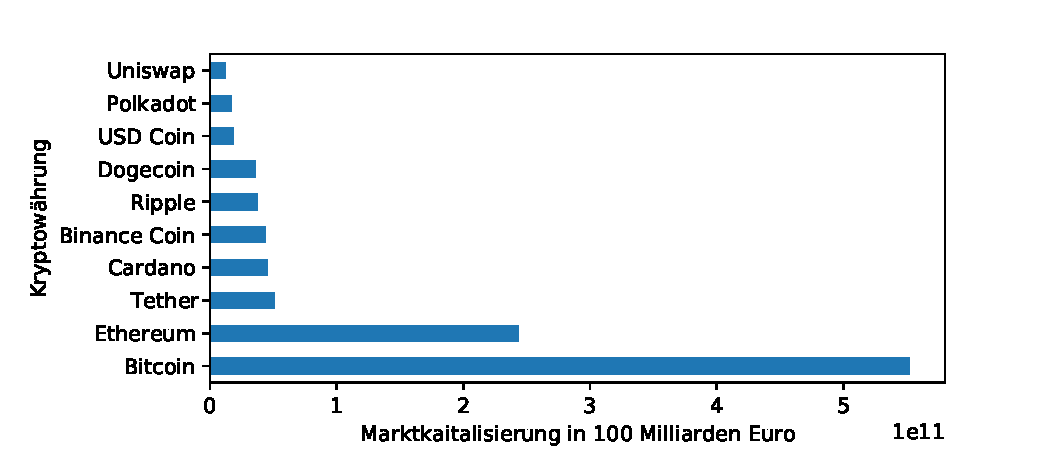
\includegraphics[scale=0.9]{./images/marketcap.pdf}
\caption{Marktkapitalisierung der Zehn größten Krytowährungen in Euro \cite{coinmarketcap}}
\centering
\end{figure}


In der folgenden Arbeit werden Funktionsweise, Chancen und Risiken sowie die wirtschaftliche Bedeutung von Kryptowährungen genauer behandelt, die Geschichte der Entwicklung wird explizit nicht thematisiert.

\section{Funktionsweise}

Die Technologie, die viele Kryprowährungen und im besonderen Bitcoin auszeichnet, ist als Blockchain bekannt. Wie der Name bereits vermuten lässt, handelt es sich dabei um eine \glqq Kette\grqq aus \glqq Blöcken\grqq in denen beispielsweise jegliche Transaktionen unter Zuhilfenahme von kryptographischen Mechanismen gespeichert sind. \cite{soeteman2019}
Die Blockchain ermöglicht es zudem, Daten nicht zentral speichern zu müssen, sonder diese dezentral in einem Peer to Peer (P2P) Netzwerk  abzulegen. In einem solchen Netz arbeiten alle Rechner, die Teil dessen sind, gleichberechtigt zusammen. Zu unterscheiden sind unterschiedliche Kryprowährungen meist in anderen Technologien,denn  so setzt Bitcoin beispielsweise zu Verifizierung der Transaktionen auf \glqq Proof-of-Work\grqq, wohingegen andere \glqq Proof-of-Stake\grqq nutzen. Weiter ist auch bemerkbar, dass Protokolle von Kryptowährungen die maximale Menge an in Umlauf befindlicher Geldmenge begrenzt können oder mal bestimmte Inflations- oder Deflationspolitik vorsehen. \cite{wegner2019}


\subsection{Blockchain am Beispiel Bitcoin}
Wie oben bereits beschrieben, verbirgt sich hinter dem Konzept der Blockchain ein Peer-to-Peer Netzwerk, und die Blockchain ermöglicht es so einen gemeinschaftlichen Konsens zu finden, ohne eine dritte zentrale Partei, wie eine Bank oder eine Regierung zu benötigen. Abbildung 2 und 3 zeigen diese Unterschiede anschaulich. 

\begin{figure}[h]
    \centering
    \begin{minipage}{0.37\textwidth}
        \centering
        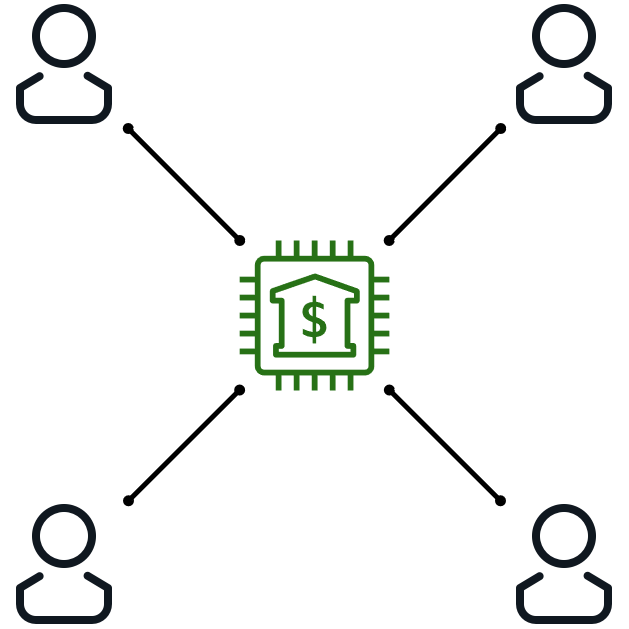
\includegraphics[width=0.7\textwidth]{./images/central.png} % first figure itself
        \caption{Bank als Zentrale Drittpartei}
    \end{minipage}
    \begin{minipage}{0.37\textwidth}
        \centering
        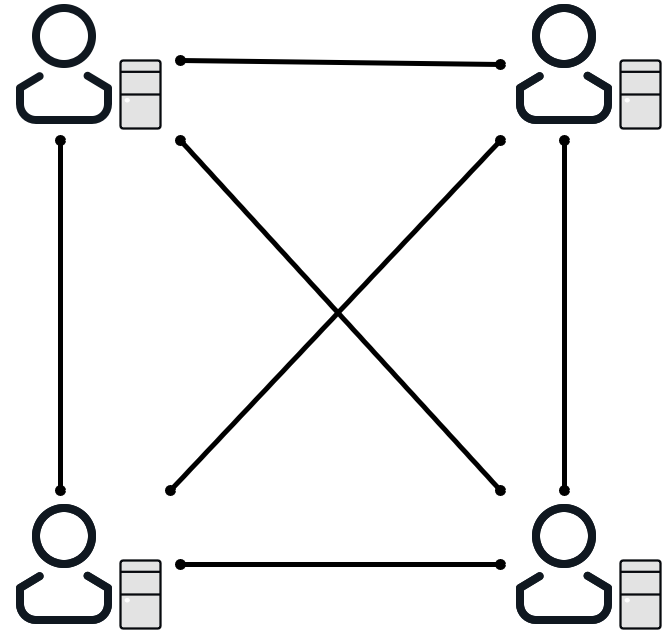
\includegraphics[width=0.7\textwidth]{./images/decentral.png} % second figure itself
        \caption{Dezentrales Peer-to-Peer Netzwerk}
    \end{minipage}
\end{figure}

Vergleicht man beide Modelle, so werden alle zentral gespeicherten Daten einer Bank wie Kontostände und Überweisungen ebenso in einer Blockchain gespeichert, nur liegen dort die Datenbanken vielfach kopiert auf allen Rechnern des Netzwerkes vor. Wichtig ist zu erwähnen, dass es sich hierbei nicht um Kopien im geläufigen Sinne handelt, sondern, da es keine Originaldatenbank gibt, jede dieser Kopien den anderen gegenüber gleichwertig ist. Da in der Blockchain alle Transaktionen gespeichert sind, fungiert das Netzwerk somit als globales und kollektives Buchführungssystem, wodurch es zudem unmöglich ist Bitcoins zu vervielfachen oder zu fälschen.
\cite{rosenberg2019}

Jeder Nutzer des Netzes ist dabei als Client anzusehen und besitzt als solcher ein Wallet, das eine digitale Analogie zur Geldbörse darstellt. In dieser Wallet jedoch sind jedoch keine Coins aufbewahrt, vielmehr ist in der Wallet ein Schlüssel gespeichert, durch welchen man zugriff auf alle Bitcoin erhalten kann, die man bisher Empfangen hat. Betätigt nun ein Client eine Transaktion, so wird diese per \glqq Best-Effort\grqq -Prinzip an alle im Netzwerk befindlichen \glqq Miner\grqq  weitergeleitet. Diese kümmern sich darum, die Transaktionen zu bestätigen und in den nächsten Block der Blockchain einfließen zu lassen.

Um dabei sicherzustellen, dass nur der rechtmäßige Besitzer die Informationen über gewollte Transaktionen seiner Bitcoins an Miner senden kann, verwendet das Protokoll der Bitcoin digitale Signaturen. Zum Zuge kommt ein asymmetrisches kryptographisches Verfahren, das mit privaten und öffentlichen Schlüsseln arbeitet, wobei beide Schlüssel nichts anderes als Zahlenkombinationen sind. Zur besseren Lesbarkeit dieser werden sie mehrmals gehashed um am Ende eine 34 stellige Zeichenkombination zu erhalten. Der private Key ist nur dem Besitzer bekannt und wird verwendet, um die eigenen Transaktionen mittels einem speziellen Algorithmus zu signieren. Der öffentliche Key ist, wie der Name bereits verrät, für jeden einsehbar und dient zur Überprüfung der Signatur einer abgesendeten Transaktion, denn ein privater und öffentlicher Schlüssel gehören immer zusammen. Somit lässt sich immer feststellen, ob bei einer Transaktion Absender und Besitzer übereinstimmen.(siehe Abb.4)
\cite{soeteman2019}\cite{binance}


\begin{figure}[h]
\centering
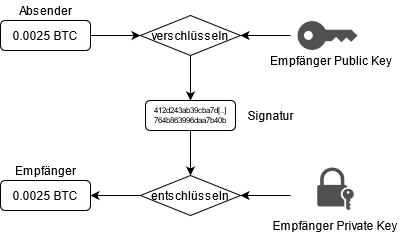
\includegraphics[scale=0.9]{./images/pubprivkey.png}
\caption{Asymmetrische Kryptographie am Beispiel einer Bitcoin Transaktion \cite{coincierge}}
\centering
\end{figure}

Wurde nun, wie tausendfach täglich, eine gültige Transaktion abgesendet, nimmt ein Miner diese in seine Version der Blockchain auf. Hier spielt nun die Dezentralisation eine große Rolle, denn alle Miner konkurrieren insgesamt darum, dass ihrer Version der Blockchain zu vertrauen ist und diese zur Fortsetzung der Blockchain verwendeter werden soll. Jeder Block der Bitcoin Blockchain hat dabei in etwa die Größe von Einem Megabyte, und ungefähr alle 10 Minuten wird der Blockchain ein neuer Block angehängt. Bevor dies allerdings geschieht, muss der Block zunächst \glqq gefunden\grqq. Im Wettkampf untereinander stellt jeder Miner zunächst seinen Block mit allen getätigten Transaktionen zusammen, und nutzt diesen dann zusammen mit zufälligen Zahlen, genannt Block Header, als Eingabe in den SHA256-Algorithmus. Ziel ist es dann durch ausprobieren verschiedenster Block-Header in der Ausgabe des Algorithmus eine bestimmte Anzahl an Nullen voranstehend zu haben. Die Genaue Anzahl an Nullen hängt dabei von der Gesamtmenge an Rechenleistung im Netz ab, denn sie ist variabel und passt sich automatisch an, um ungefähr bei Zehn Minuten Rechenzeit pro Block zu bleiben. \cite{fraunhofer2019}

Wurde von einem Miner dann eine Korrekte Zahl gefunden verkündet dieser es im Netzwerk und die restlichen Geräte überprüfen den Hash des Blocks mit Hilfe des Block-Headers und zudem, ob auch alle Transaktionen im Block korrekt sind. Ist er gültig, übernehmen sie ihn. Als Belohnung für die geleistete Rechenarbeit erhält der Miner, dessen Block übernommen wird, als Belohnung eine vordefinierte Menge Bitcoin, die vorher noch nicht existierten, und zudem die Summe aller Transaktionsgebühren der im Block enthaltenen Transaktionen. \\

Um Manipulationen von Transaktionen in früheren Blöcken zu verhindern, beinhaltet ein Block immer auch den Hash des vorherigen Blocks. Ändert man also den Inhalt eines früheren Blocks, so ändert sich damit auch dessen Hash, und der aller darauf folgenden Blöcke in einen ungültigen Hash. Diese \glqq Verkettung\grqq aller Blöcke führt zu dem Namen Blockchain. \cite{rosenberg2019}

\subsection{Proof of Work vs Proof of Stake}
Das oben beschriebene Konzept, wie es beispielsweise von den Kryptowährungen Bitcoin und Litecoin angewandt wird, nennt sich auch \glqq Proof-of-Work\grqq (PoW), denn für die Verifizierung der Legitimität (Proof) von Transaktionen müssen Berechnungen (Work) durchgeführt werden. Welche Ausmaße das aufgrund der Lukrativität des Bitcoin schürfen angenommen hat, verdeutlicht Abbildung 5.
\begin{figure}[h]
\centering
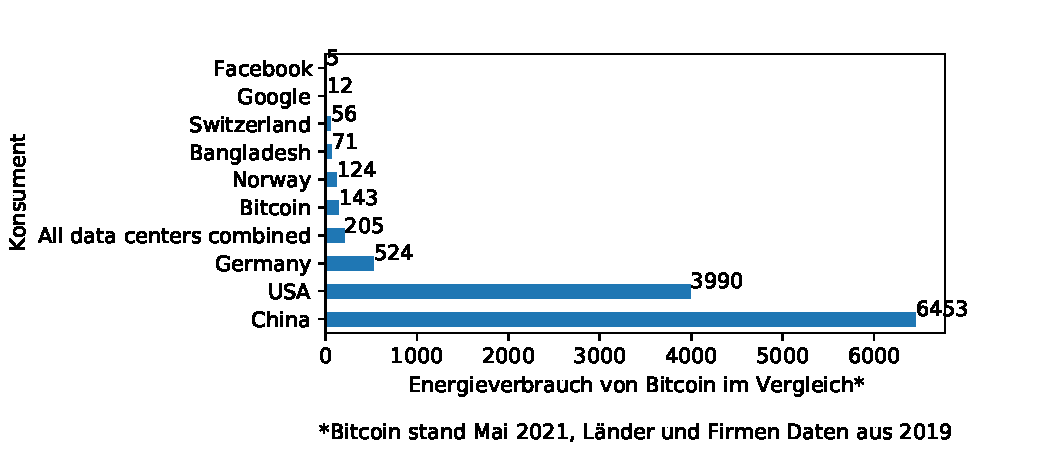
\includegraphics[scale=0.7]{./images/energyconsume.pdf}
\caption{Stromverbrauch des Bitcoin-Netzwerkes im Vergleich zu anderen Konsumenten \cite{statista2021}}
\centering
\end{figure}

Wie sich unschwer erkennen lässt übersteigt der Energiebedarf des Bitcoin Minings inzwischen sogar den ganzer Länder, und im Vergleich zu IT-Riesen ist deren Energieverbrauch marginal. Da inzwischen in jeder Gesellschaftlichen Schicht jedoch klar wird, dass wir eine kommende Katastrophe die durch immer steigende Temperaturen dringlichst zu verhindern haben, wird die Kritik immer lauter. Ein Lösungsvorschlag hierbei lautet Proof-of-Stake, denn anders als bei PoW werden hier keine Berechnungen mehr benötigt. Es handelt sich dabei weitgehend um das selbe Konzept, nur dass anstelle des Arbeitens Sicherheiten in Form des jeweiligen Coin hinterlegt werden müssen und über den Zeitraum des Minings eingefroren bleiben. Mit diesem Anteil an eingefrorener Währung validiert ein Nutzer dann ebenso die Transaktionen für einen Block. Wer aus dem Pool aller Miner im Endeffekt ausgewählt wird, den Block zu validieren ist dabei in einem zuvor festgelegtem Algorithmus beschrieben und sollte möglichst Zufällig sein. Je nach Implementierung bekommen die Miner dann beispielsweise die transaktionsgebühren alles Transaktionen des verifizierten Block oder etwa jähliche Zinsen auf die eingefrohrenen Coins. \cite{soeteman2019}
\subsection{Ethereum und Smart Contracts}

Ethereum belegt gemessen an der Marktkapitalisierung den zweiten Platz aller Kryptowährungen, weswegen sich ein kurzer Blick hierauf lohnt. Im Vergleich zu Bitcoin scheint Ethereum zunächst sehr ähnlich zu sein, denn beide Protokolle verwenden eine Blockchain in Kombination mit Proof-of-Work, doch Ethereum ist mehr als eine reine Kryptowährung. In erster Linie ist Ethereum eine Plattform für die Entwicklung dezentraler Apps über sogenannte Smart Contracts. Ein solcher Smart Contract kann dabei von einem dezentralen Wahlsystem, über Kredite und Versicherungen bis hin zu Crowdfunding reichen. Hier ist auch von Vorteil, dass Ethereum Transaktionen deutlich schneller und günstiger verarbeiten kann als in Bitcoin. Der Konsens des Ethereum-Netzwerks ist zudem auf der Seite des Wechsels zu einem System dass auf Proof-of-Stake aufbaut, Test-Netzwerke sind bereits am laufen und der Wechsel des Hauptnetzes soll noch 2021 stattfinden. \cite{soeteman2019} \cite{eth2021}

\section{Wirtschaftliche Bedeutung}



\subsection{Kursentwicklung}

Seit Veröffentlichung des Bitcoin Protokolls im Jahre 2009 erlebt deren Kurs wiederholtes immenses Wachstum mit nachgefolgtem Absturz. Erhielt man zu Beginn ein Bitcoin für circa 0,0007 Euro, so musste man ein Jahr später schon 0,07 Euro dafür bezahlen, was zu einem immenser Wertsteigerung von 1000\% führt! Die führte sich lange so fort, 2011 wuchs der Wechselkurs von 1 Euro auf 20 Euro, gefolgt von einem ersten Crash auf 10 Euro in folge eines Hackerangriffs. Über die Jahre verbreiteten sich Bitcoin und Kryptowährungen immer weiter, das mag an dem aus der Finanzkrise noch immer fehlendem Vertrauen in Banken, dem Lockruf vermeintlicher Gewinne oder der Überzeugung die zentralen Geldinstitute abzuschaffen liegen. 

\begin{figure}[h]
\centering
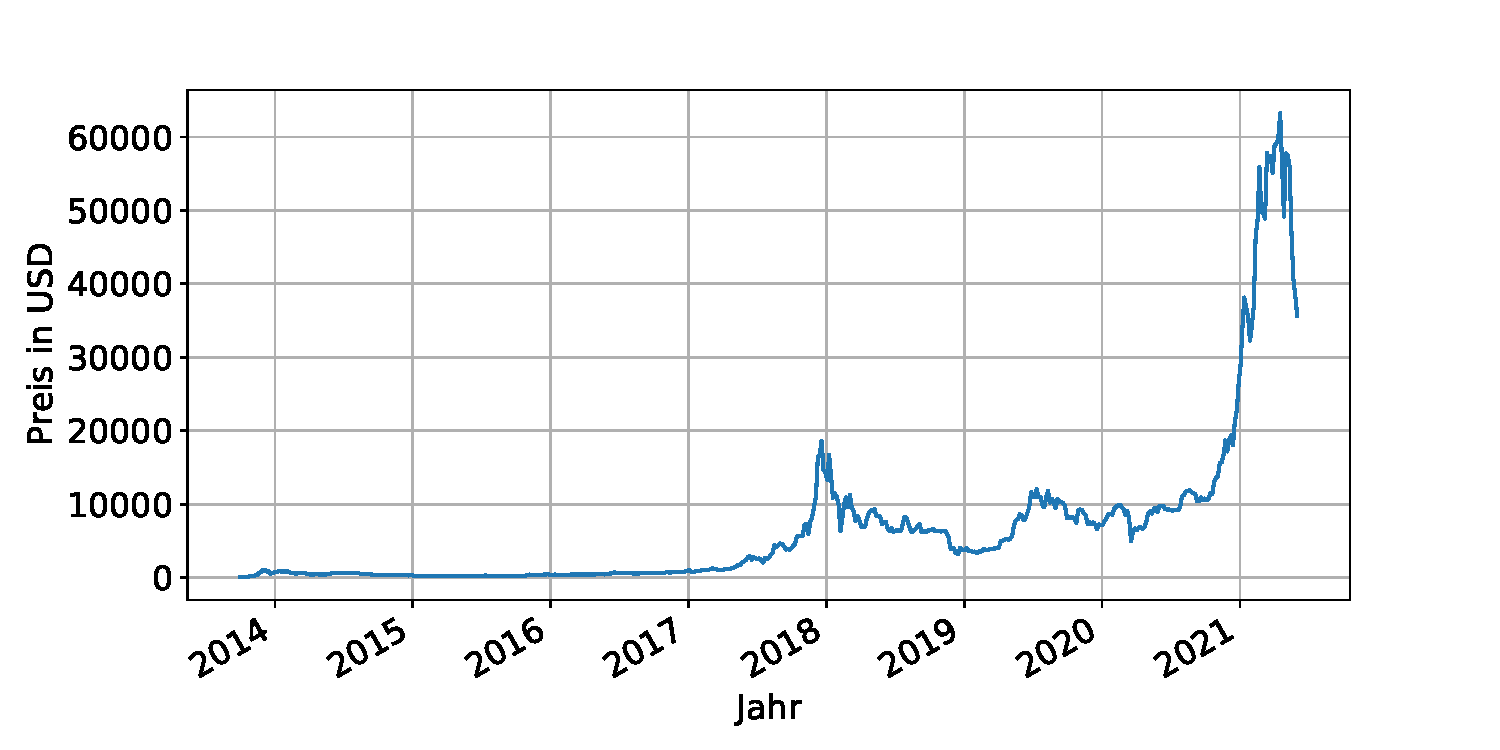
\includegraphics[width=0.9\textwidth]{./images/btcchart.pdf}
\caption{Wechselkurentwicklung von Bitcoin seit 2014 \cite{coindesk2021}}
\centering
\end{figure}

Dies spiegelt sich auch in der Wertentwicklung dieser Währungen wieder, exemplarisch sieht man den Wechselkurs von Bitcoin in Abbildung 6. Nicht zuletzt hat Bitcoin neue Höchststände erreicht, und ist in den darauffolgenden Wochen erneut um über 25\% abgestürzt. Doch lässt sich das nicht nur über Bitcoin sagen, denn der gesamte Kryptowährungsmarkt ist diesem Kurs gefolgt. Kryptowährungen haben sich inzwischen als Wertanlage etabliert, wenn auch eine gewisse Risikobereitschaft vorliegen sollte.\cite{coinmarketcap}
\subsection{Risiken}

\subsubsection{Die 51\% Attacke}

Wie bereits beschrieben ist es beim Mining von neuen Blöcken notwendig, den Konsens aller im dezentralen Netzwerk befindlichen Miner zu erhalten. Wäre es nun so, dass ein einziger Miner über 50\% aller Rechenleistung bereitstellen kann, ist dieser in der Lage böswillig Transaktionen rückgängig zu machen, was zum doppelten Ausgeben dieser Coins führen kann. Zudem kann verhindert werden, dass einige oder alle Transaktionen bestätigt werden. 

Diese Szenario jedoch ist relativ unwahrscheinlich, da ein solcher Angriff wenig lukrativ und eher sehr Kostenintensiv ist und hauptsächlich dazu führen würde, den Kurs einer Kryprowährung stark zu vermindern oder die Kryptowährung komplett zu zerstören. \cite{binance2020}

\subsubsection{Überlastung}

Besonders in Hochzeiten von Kryptowährungen steigen Transaktionskosten ins Unermessliche da sehr viele Transaktionen getätigt werden, und um diese so schnell wie möglich im nächsten Block validiert zu bekommen, werden teils freiwillig höhere als übliche Transaktionsgebühren abgegeben, was zu allgemein steigenden Gebühren führt. Beispielsweise musste man 2017 umgerechnet teils 10 € Transaktionsgebühren für eine Bitcoinüberweisung zahlen, selbst wenn diese selbst nur einen Betrag von umgerechnet 5 € betrug. Dies liegt an der Begrenzten Größe der Blöcke und der festgelegten Dauer von 10 Minuten pro Block. 


\begin{figure}[h]
\centering
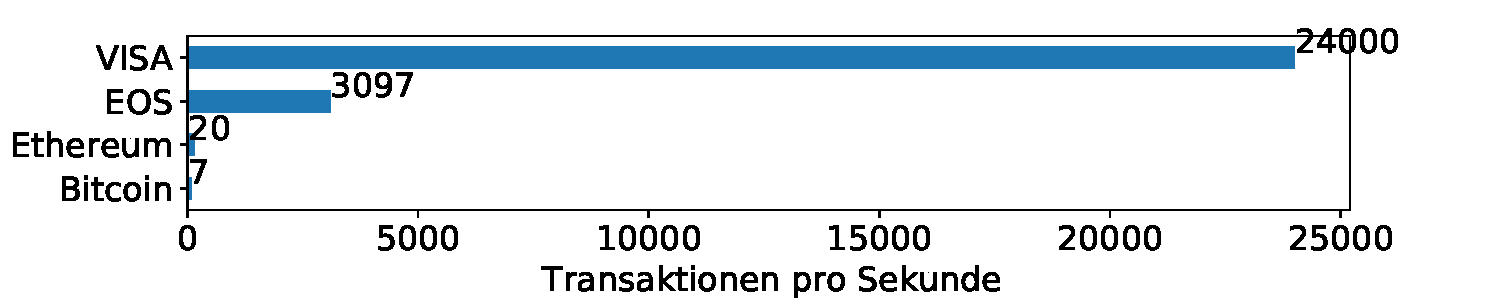
\includegraphics[width=0.9\textwidth]{./images/transactions.pdf}
\caption{Maximales Transaktionsvolumen pro Sekunde im Vergleich \cite{rosenberg2019}}
\centering
\end{figure}

Im direkten Vergleich mit dem Zahlungsdienstleister Visa scheinen Kryptowährungen meilenweit abgehängt zu sein, doch dreht es sich bei der Statistik in Abbildung 7 um die maximale Kapazität. Visa bearbeitet normalerweise maximal 1700 Transaktionen pro Sekunde, und das erreicht EOS mit 3000 pro Sekunde ebenso. Ein Ansatz um Bitcoin und Ethereum Transaktionen schnelle und günstiger zu gestalten wäre Blockgröße zu erhöhen, was bei Bitcoin beispielsweise schon getan wurde.\cite{rosenberg2019}

\subsubsection{Kriminalität}

Kryptowährungen sind ein häufig genutztes Mittel unter Kriminellen. Lösegeldforderungen bei verschlüsselten IT-Systemen oder im realen Leben bei Geiselnahmen sind schon länger Gang und Gäbe. Weiter wird auf digitalen Schwarzmarktplattformen nur in Kryptowährungen bezahlt, dort reichen Verkaufsangebote von Drogen über Waffen bis hin zu Auftragsmorden oder Menschenhandel. Der Grund hierfür liegt auf der Hand: Vermeintliche Anonymität die keiner Behörde die Nachverfolgung von Käufer oder Verkäufer ermöglicht. Nichtsdestominder muss man hier anmerken, dass nur ein marginaler Teil aller Transaktion tatsächlich kriminellen Ursprungs sind.

Smart Contracts bieten zudem die Möglichkeit zum Beispiel ein Programm zu entwickeln, in dem ein Auftragsmord an einen Politiker entlohnt wird. Das Programm kann dann ebenfalls nicht nachverfolgt werden, da es eben dezentral gespeichert wird.  

\subsubsection{Weitere Risiken}
Ohne genauer darauf einzugehen sind hier weitere mögliche Risiken die Kryptowährungen begegnen aufgelistet: 

\begin{itemize}
  \item \textbf{Verlustrisiko:} Der Wert kann aufgrund verschiedener Szenarien auf Null fallen
  \item \textbf{Verbotsrisiko:} Autoritäre Regierungen können ein Verbot von Kryptowährungen durchsetzten.
  \item \textbf{Kontrollrisiko:} Open-Source und Dezentralisierung machen Kontrollen unmöglich
  \item \textbf{Deflationsrisiko:} Dies ist aufgrund der technischen Begrenzung der in Umlauf befindlichen Coins einiger Kryptowährungen. 
  \item \textbf{Regulierungsrisiko:} Durch staatliche Regulierung von Finanzprodukten könnten Unternehmen die mit Bitcoin handeln starke Regulierungen erfahren.
\end{itemize}\cite{neumann2017}

\subsection{Chancen}

\subsubsection{Grenzenlose Währung}
Prinzipiell sind Kryptowährungen global und ohne Einschränkungen nutzbar. Einzig die Verbreitung einer Währung hat einen Einfluss darauf, ob man denn nun einen Handelpartner findet, der die gewünschte Währung auch unterstützt.

\subsubsection{Sicherheit in Krisenzeiten}
Kryptowährungen sind aktuell besonders in Ländern mit instabilen Währungen und hoher Inflation sehr akzeptiert, um so dem Wertverlust des angesparten zu verhindern. Betrachtet man Venezuela mit Inflationsraten von über 13.000\%, ist es wohl trotz hoher Volatilität im Kryptomarkt kaum möglich sein Geld dort schneller zu verlieren. Ebenso erfahren Kryptowährungen in politisch instabilen Ländern mit hoher Korruption hohe Beliebtheit, da so Staaten- und Bankenunabhängig über das eigene Vermögen verfügt werden kann. \cite{rosenberg2019}

\subsubsection{Smart Contracts}

Smart Contracts bietet als Protokoll, das automatisch zuvor festgelegte Aktionen ausführt, eine Plattform die kein Vertrauen mehr voraussetzt. Das Versicherungsunternehmen AXA hat beispielsweise mit einer Versicherungen für Flugverspätungen experimentiert, die automatisch Flugdaten eingelesen hat und im Falle einer entstandenen Verspätung die festgelegte Versicherungssumme auszahlte. \citep{hmd2019}

\section{Ausblick}

Kryptowährungen stellen eine Technologie dar, die das Potenzial bieten unsere Gesellschaft zu verändern. Mit Anbeginn des Internets wurde Sektor um Sektor digitalisiert, das Online-Banking ist inzwischen zu einem Hauptbestandteil des Lebens vieler Menschen geworden. Kryptowährungen habe sich dieses Vertrauen noch zu erarbeiten, Funktionalität und allgemeine Vorteile gegenüber der klassischen Finanzsysteme sollten in den vorangegangenen Kapiteln deutlich geworden sein, auch wenn sie noch immer wegen vermeintlicher illegaler Zusammenhänge mit einem schlechten Ruf zu kämpfen haben.

Zusätzlich zum allgemeinen Nutzen als Zahlungsmittel sind Kryptowährungen zuletzt immer weiter ins Auge von Anlegern gerückt. Die fortschreitende Nutzung und Bekanntheit wird auf lange Sicht dazu führen, dass auch die Akzeptanz als Zahlungsmittel in analogen Läden zunimmt.

Experten aus allen Branchen sehen Kryptowährungen bereits jetzt als Erfolg an und halten an deren Überlegenheit gegenüber Fiatgeld fest, was der Börsenkurs von Bitcoin und Co. durchgängig bestätigen. So war es auch die Intention des Erfinders der Bitcoin, Satoshi Nakamoto, eine Alternative zum bisherigen Finanzsystem aufzuzeigen, und sollte der bisherige Spitzenreiter Bitcoin doch einmal verschwinden, so hinter bleibt ein Gedanke, der in vielen anderen Kryptowährungen halt gefunden hat.
%%%%%%%%%%%%%%%%%%%%%%%%%%%%
%% Literaturverzeichnis wird 
%% automatisch eingefügt
%%%%%%%%%%%%%%%%%%%%%%%%%%%%
\clearpage
\lhead{}
\printbibliography
\addcontentsline{toc}{section}{\bibname}


%%%%%%%%%%%%%%%%%%%%%%%%%%%%
%% Eidesstattliche Erklärung
%% muss angepasst werden 
%% in Erklaerung.tex
%%%%%%%%%%%%%%%%%%%%%%%%%%%%
\newpage
\begin{otherlanguage}{ngerman}
\thispagestyle{empty}
\section*{Eidesstattliche Erklärung}
\thispagestyle{empty}
Hiermit versichere ich, die vorliegende Arbeit selbstständig verfasst und keine anderen als die angegebenen Quellen und Hilfsmittel benutzt sowie die Zitate deutlich kenntlich gemacht zu haben.
\newline
Ich erkläre weiterhin, dass die vorliegende Arbeit in gleicher oder ähnlicher Form noch nicht im Rahmen eines
anderen Prüfungsverfahrens eingereicht wurde.
\vspace{4\baselineskip}\\
Stuttgart, den \today \hfill
 \includegraphics[width=0.3\textwidth]{./images/unterschrift.png}
\vspace{4\baselineskip}\\
\end{otherlanguage}

\end{document}
